\documentclass[accentcolor=tud6b,colorbacktitle,inverttitle,landscape,german,presentation,t]{tudbeamer}
\usepackage{ngerman}

\usepackage[utf8]{inputenc}

\begin{document}
	
	\title[Freifunk-Firmware Testframework]{Freifunk-Firmware Testframework}
	\subtitle{BSc Praktikum WiSe 2015/16}
	
	\author{Ana Barroso}
	\institute{Chaos Darmstadt e.V.}
	
	\logo{\url{darmstadt.freifunk.net}}
	% \logo{\color{tudtextaccent}\large IFP}
	
	\date{\today}
	
	\begin{titleframe}
		\begin{center}
			\vspace{1.5cm}
			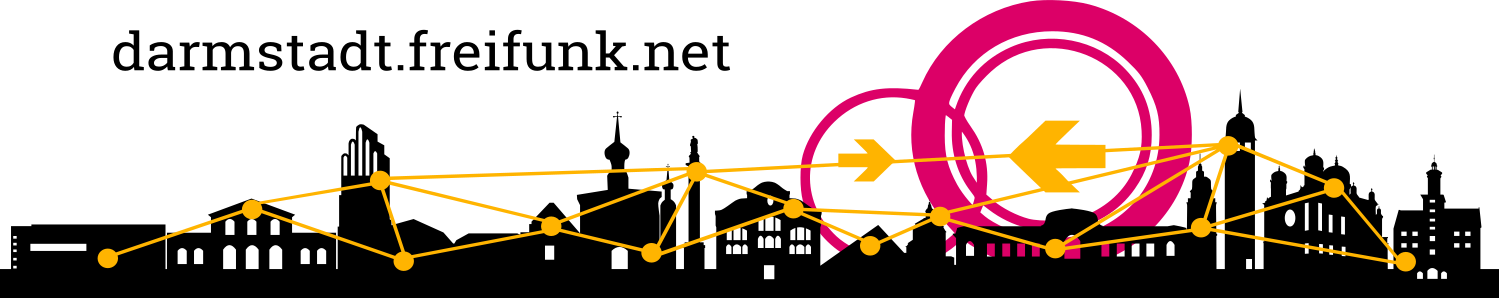
\includegraphics[width=0.7\textwidth]{images/logo-skyline}
			\vspace{1.4cm}
		\end{center}
			\flushright
			
\includegraphics[width=0.15\textwidth]{images/cda}
	\end{titleframe}
	
	\begin{frame}
		\frametitle{Einleitung}
		Freifunk:
		\begin{itemize}
			\item nichtkommerzielle Initiative
			\item Ziel: Aufbau und Betrieb eines freien WLAN-Meshnetzes
			\item dezentrales Netz besteht aus den Routern vieler einzelner Betreiber
			\item ca. 20.000 Freifunk-Router in Deutschland
			\item OpenWrt basierte Firmware von lokalen Enthusiasten entwickelt
		\end{itemize}
		\vfill
		\pause
		Um die Qualität der ausgelieferten Firmware über Releases hinweg sicherzustellen ist es notwendig diese vor dem Ausrollen ausführlich auf verschiedenen Modellen zu testen. Diese mühsame und zeitaufwendige Prozedur soll in diesem Projekt automatisiert werden.
	\end{frame}
	
	\begin{frame}
		\frametitle{Aufgabenstellung (1/2)}
		    Konstruktion eines Testframeworks, das SOHO-Router mit einer Firmware flashed,
		    konfiguriert und anschließend testet.
		    \vfill
		    Hierzu wird die folgende Hardware bereitgestellt:
		    \begin{itemize}
			    \item Managed Switch, 16 Port
			    \item regelbare Steckdosenleiste (z.B. Ubiquiti mPower)
			    \item Embedded ARM-Board, z.B. RasPi2 (Controller)
			    \item WLAN-Adapter 802.11ac
		    \end{itemize}
	\end{frame}
	
	\begin{frame}
		\frametitle{Aufgabenstellung (2/2)}
		\vfill
		Realisierung
		\begin{itemize}
			\item für Debian-basierte Linuxdistributionen (z.B. Raspbian)
			\item mit Python 3 (>=3.3) nach gängigen Standards (z.B. PEP8)
			\item unter Revisionskontrolle mit Git und sprechenden Commit-Messages\footnote{vgl. \url{http://chris.beams.io/posts/git-commit/}}
			\item lizensiert unter MIT, LGPL oder vergleichbaren Lizenzen
		\end{itemize}
		\vfill
		Die Kommunikation mit den Routern erfolgt im Regelfall per Telnet/SSH bzw. in späteren Ausbaustufen auch per tftp (Recovery, Image flashen) bzw. HTTP (Konfiguration/Ersteinrichtung über
		Weboberfläche).
		\vfill
	\end{frame}
	
	\begin{frame}
		\frametitle{Setup}
			\begin{itemize}
			    \item Bis zu 6 SOHO Router
		    	\item LAN- und WAN-Port mit einem Managed Switch verbunden
			    \item LAN per Trunk, getagged an den Controller (RasPi2) angebunden
			    \item WAN mit Dual-Stack Internet-Anbindung
			    \item VLAN und ggf. Network Namespaces auf Controller
		    \end{itemize}
			\vfill
	\end{frame}

	\begin{frame}
		\frametitle{Funktionsumfang (1/2)}
		\begin{itemize}
			\item Hardwareerkennung (Model, Revision, Primäre MAC-Addresse)
			\item Ansteuerung der Steckerleiste
			\item Weboberfläche zur Steuerung und Überwachung der Tests:
			\item Tests für einzelne Geräte starten/stoppen
			\item Auswahl und Flashen der zu testenden Firmware
			\item Auszuführende Tests auswählen
			\item Möglichkeit Tests abzubrechen
			\item Statusübersicht über laufende Tests
			\item Ergebnisreport
			\item Kaltstart der Geräte
			\item Erkennung von Software-Defekten und Firmware-Recovery
			\item Fernsteuerung und Ausführung der Tests per SSH
		\end{itemize}	
	\end{frame}
	
	\begin{frame}
		\frametitle{Funktionsumfang (2/2)}
		\begin{itemize}
			\item Testumfang:
			\item Vorbedingung(en)
			\item Aktion
			\item Erwartung
			\item Timeout
			\item Logging
			\item Ergebnis
			\item Automatischer Abruf neuer Firmware-Images vom Buildserver
			\item Unattended Betriebsmodus
			\item Ergebnisreport per Email
			\item Archivierung von Testberichten und Logdateien (syslog, dmesg)
		\end{itemize}	
	\end{frame}
	
	\begin{frame}
		\frametitle{Beispielhafte Tests}
		\begin{itemize}
		    \item Durchlaufen des Konfigurationsassistenten
		    \item Log-Prüfung, z.B. auf Kernel Panics
		    \item Autoupdater
		    \item Verbindung als WLAN-Client
		    \item Erkennung von Mesh-Verbindungen
		    \item Prüfung auf IPv6-Konnektivität
		    \item Gateways
		    \item Update-Server
		    \item NTP
		    \item Internet
		    \item Überprüfung auf laufende Dienste
		    \item Überprüfung auf NTP-Synchronisierung
 		\end{itemize}
	\end{frame}
\end{document}